\documentclass[12pt,a4paper]{report}
\usepackage{geometry}
\usepackage{titlesec}
\usepackage{needspace}
\usepackage{microtype}
\usepackage[none]{hyphenat}
\usepackage{amsmath}
\usepackage{graphicx}
\usepackage{caption}
\usepackage{setspace}
\usepackage{cite}
\usepackage{lipsum}
\usepackage{float}
\usepackage{enumitem}
\usepackage{hyperref}
\usepackage{times}           % For Times New Roman text
\usepackage{mathptmx}        % For Times New Roman math symbols
\usepackage[T1]{fontenc}
\usepackage{ragged2e}
\usepackage{microtype}
\setlength{\parindent}{1em}
\setlength{\parskip}{1ex}
\justifying


\microtypesetup{
    stretch=10,
    shrink=10,
    step=1
}
\geometry{top=2.5cm, bottom=2.5cm, left=2.5cm, right=2.5cm, headheight=1cm, footskip=1cm}
\setstretch{1.5}
\titleformat{\chapter}[hang]{\normalfont\huge\bfseries}{\thechapter.}{12pt}{}
\titleformat{\section}[hang]{\normalfont\Large\bfseries}{\thesection.}{6pt}{}
\titleformat{\subsection}[hang]{\normalfont\large\bfseries}{\thesubsection.}{6pt}{}
\titleformat{\subsubsection}[hang]{\normalfont\normalsize\bfseries}{\thesubsubsection.}{6pt}{}
\titlespacing*{\chapter}{0pt}{24pt}{12pt}
\titlespacing*{\section}{0pt}{24pt}{12pt}
\titlespacing*{\subsection}{0pt}{12pt}{6pt}
\titlespacing*{\subsubsection}{0pt}{12pt}{6pt}
\hyphenpenalty=10000        % Discourage hyphenation
\exhyphenpenalty=10000  
\captionsetup{font=small,labelfont=bf,justification=centering}
\setcounter{chapter}{0}  % Ensure chapters start at 1
\setcounter{section}{0}
\titleformat{\chapter}[hang]
{\normalfont\huge\bfseries}
{Chapter \thechapter:}{12pt}{\huge}
\sloppy
\widowpenalty=10000
\clubpenalty=10000
\raggedbottom
\begin{document}
\chapter*{Acknowledgments}
\addcontentsline{toc}{chapter}{Acknowledgments}
\markboth{Acknowledgments}{}

I would like to express my sincere gratitude to my supervisor, Mr. Adel Ayari, for his guidance and support throughout the internship. I am grateful for his valuable feedback and advice, which have been instrumental in the successful completion of this project.

I am particularly thankful to Mr. Zino Abidi for guiding me through Playwright integration and sharing valuable insights on CI/CD workflows, which were instrumental in completing my tasks.

I would like to also thank my colleagues at the company for their help and support during the internship. I am grateful for their assistance and collaboration, which have made this internship a rewarding and enriching experience.

\chapter*{List of Abbreviations}
\begin{description}[leftmargin=*, widest=DCCHTM]
    \item[QA] Quality Assurance
    \item[CI/CD] Continuous Integration/Continuous Deployment
    \item[E2E] End-to-End
    \item[UX/UI] User Experience/User Interface
    \item[VAT] Value-Added Tax
    \item[BVA] Boundary Value Analysis
    \item[EP] Equivalence Partitioning
\end{description}

\tableofcontents
\listoffigures


\chapter*{Introduction}
\addcontentsline{toc}{chapter}{Introduction}
\markboth{Introduction}{}

This report presents the work carried out during the internship at SeekMake for a duration of two months.

The internship was focused on software testing and quality assurance of the SeekMake web application. It covers the testing journey from exploratory testing to end-to-end testing and automation.

The report is divided into four chapters:

\begin{itemize}
    \item \textbf{Chapter 1: Company Overview} provides an introduction to SeekMake, a leading provider of digital transformation services.
    \item \textbf{Chapter 2: Quality Assurance Framework} covers the basics of software testing and quality assurance, including the testing lifecycle and methodologies.
    \item \textbf{Chapter 3: Exploratory Testing Insights} discusses the exploratory testing carried out during the internship.
    \item \textbf{Chapter 4: End-to-End Testing and Automation} discusses the end-to-end testing and automation of the SeekMake web application.
\end{itemize}

\chapter{Company Overview}
\markboth{Company Overview}{}

\section{About SeekMake}
SeekMake, a leading provider of digital transformation services, specializes in streamlining manufacturing processes through its comprehensive online platform. Key offerings include instant quoting, CAD tools, secure file storage, and analytics, all designed to reduce development cycles and enhance project delivery speed. These services empower manufacturers to manage production, customer interactions, and payments efficiently through an intuitive web interface. \cite{seekmakefeatures}
\begin{figure}[H]
    \centering
    
\includegraphics{project/images/seekmake.png}
    \caption{SeekMake Logo}
    \label{fig:seekmake-logo}
\end{figure}

\begin{figure}[H]
    \centering
    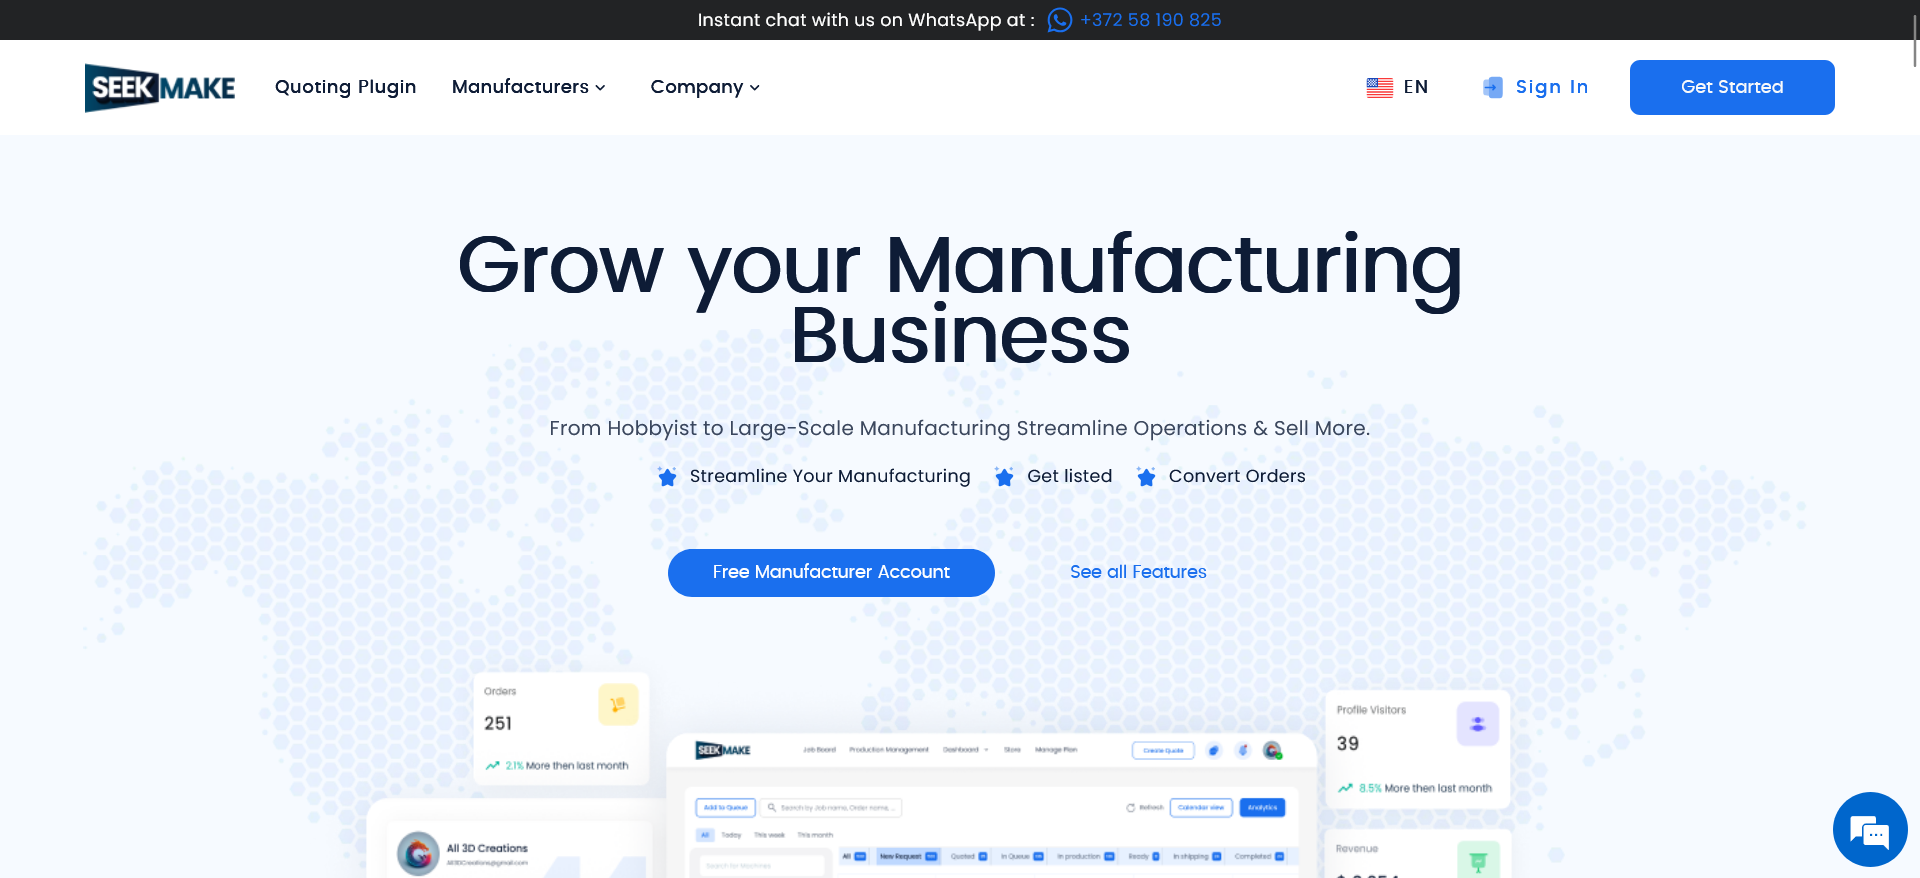
\includegraphics[width=\textwidth]{project/images/seekmake-homepage.png}
    \caption{A screenshot of SeekMake's homepage}
    \label{fig:seekmake-homepage}
\end{figure}
\chapter{Quality Assurance Framework}
\markboth{Quality Assurance Framework}{}

\section{Introduction}

This chapter presents the quality assurance framework used during the software testing process at SeekMake.

It covers quality assurance vs testing, the Scrum methodology, the integration of DevOps, testing strategy, testing types, testing tools, and testing techniques used to ensure the quality of the software.

\section{Quality Assurance vs Testing}

While people often use the terms “testing” and “quality assurance” (QA) interchangeably, testing and QA
are not the same \cite{istqbctfl4.0.1}:

\subsection{Quality Assurance}

QA is a process-oriented, preventive approach that focuses on the implementation and improvement of
processes. It works on the basis that if a good process is followed correctly, then it will generate a good
product. \cite{istqbctfl4.0.1}

QA at SeekMake guided the testing process by defining the testing strategy, planning the testing activities, and ensuring that the testing activities were aligned with the sprint goals.

\subsection{Software Testing}

Testing is a product-oriented, corrective approach that focuses on those activities supporting the
achievement of appropriate levels of quality. \cite{istqbctfl4.0.1}

Testing at SeekMake was carried out to identify and fix defects\footnote{A defect is an error, flaw, failure, or fault in a computer program that causes it to produce an incorrect or unexpected result, or to behave in unintended ways} in the web application. This corrective approach was complemented by QA activities that focused on process improvement and defect prevention.

\subsection{Differences and Complementarity}

Test results are used by QA and testing. In testing they are used to fix defects, while in QA they provide
feedback on how well the development and test processes are performing. \cite{istqbctfl4.0.1}

\section{Scrum Methodology}

At SeekMake, the testing process was aligned with the Scrum methodology.

\subsection{Scrum Overview}

Scrum helps people and teams deliver value incrementally in a collaborative way. As an agile framework, Scrum provides just enough structure for people and teams to integrate into how they work, while adding the right practices to optimize for their specific needs. \cite{scrum}

At SeekMake, Scrum was used to manage the testing process, ensuring that the testing activities were aligned with the sprint goals and that the testing process was integrated with the development activities.
\subsection{Scrum Team}

The fundamental unit of Scrum is a small team of people, a Scrum Team. The Scrum Team consists of one Scrum Master, one Product Owner, and Developers. \cite{scrum}

At SeekMake, the Scrum Team consisted of developers (including QA testers and UX/UI designers), a product owner, and a Scrum master.
\subsubsection{Scrum Master}

the Scrum Master is accountable for establishing Scrum. They do this by helping everyone understand Scrum theory and practice, both within the Scrum Team and the organization while serving the Scrum Team as well as the larger organization. \cite{scrum}

\subsubsection{Product Owner}
The Product Owner is accountable for maximizing the value of the product resulting from the work of the Scrum Team. How this is done may vary widely across organizations, Scrum Teams and individuals. \cite{scrum}

\subsubsection{Developers}
Developers are the people on the Scrum Team that are committed to creating any aspect of a usable Increment each Sprint.\cite{scrum}

\subsection{Scrum Events}

Each event in Scrum is a formal opportunity to inspect and adapt Scrum artifacts. These events are specifically designed to enable the transparency required. Failure to operate any events as prescribed results in lost opportunities to inspect and adapt. Events are used in Scrum to create regularity and to minimize the need for meetings not defined in Scrum. \cite{scrum}

\subsubsection{Sprints}

Sprints are fixed length periods of work that last one month or less to create consistency and ensure short iterations for feedback in order to inspect and adapt both how work is done and what is being worked on. \cite{scrum}

At SeekMake, sprints lasted two weeks and were used to define the scope of the testing activities, assign tasks to team members, and estimate the effort required to complete the testing activities.

\subsubsection{Sprint Planning}

Sprint Planning initiates the Sprint by laying out the work to be performed for the Sprint. This resulting plan is created by the collaborative work of the entire Scrum Team. \cite{scrum}

\subsubsection{Daily Scrum}

The Daily Scrum (or daily Stand-Up) is a 15-minute event for the Developers of the Scrum Team. To reduce complexity, it is held at the same time and place every working day of the Sprint. \cite{scrum}

At SeekMake, daily stand-ups were used to share updates, collaborate on testing activities, and resolve issues.

\section{Integration of DevOps}
At SeekMake, the testing process was integrated with DevOps practices to ensure that the testing activities were aligned with the development activities.

\subsection{DevOps Overview}

DevOps is an organizational approach aiming to create synergy by getting development (including
testing) and operations to work together to achieve a set of common goals. \cite{istqbctfl4.0.1}

\begin{figure}[H]
    \centering
    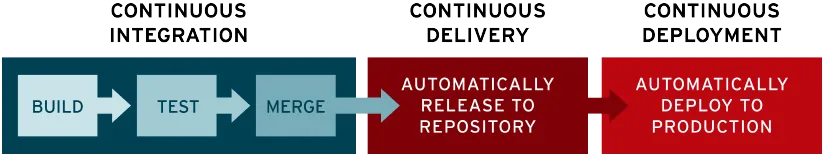
\includegraphics[width=\textwidth]{project/images/ci-cd-flow-desktop.png}
    \caption{DevOps practices.}
    \label{fig:devops-practices}
\end{figure}

\subsubsection{Continuous Integration}

Continuous integration (CI) is the practice of automating the integration of code changes from multiple contributors into a single software project. It’s a primary DevOps best practice, allowing developers to frequently merge code changes into a central repository where builds and tests then run. Automated tools are used to assert the new code’s correctness before integration. \cite{atlassian}

\subsubsection{Continuous Delivery}

Continuous delivery is an extension of continuous integration since it automatically deploys all code changes to a testing and/or production environment after the build stage.\cite{atlassian}

\subsubsection{Continuous Deployment}

Continuous deployment goes one step further than continuous delivery. With this practice, every change that passes all stages of your production pipeline is released to your customers. There's no human intervention, and only a failed test will prevent a new change to be deployed to production. \cite{atlassian}

\section{Testing Strategy}
The testing strategy outlines the approach that was adopted during the software testing process at SeekMake. It includes the testing objectives, scope, and resources required to carry out the testing activities.

\subsection{Testing Objectives}
The primary testing objectives were to ensure seamless user experiences by validating the core functionalities of SeekMake’s web application. Specific goals included verifying the checkout workflow, ensuring secure payment processing, and assessing the application’s compatibility across major browsers and devices.

\subsection{Testing Scope}
The testing scope included the following areas of the web application:

\begin{itemize}
    \item \textbf{Functionality:} Verify that the web application functions as expected.
    \item \textbf{Performance:} Evaluate the performance of the web application under different conditions.
    \item \textbf{Usability:} Assess the usability of the web application from an end-user perspective.
    \item \textbf{Compatibility:} Test the web application on different devices and browsers to ensure compatibility.
    \item \textbf{Security:} Identify and address security vulnerabilities in the web application.
\end{itemize}

\subsection{Testing Resources}
The testing resources required to carry out the testing activities included the following:

\begin{itemize}
    \item \textbf{QA Testers:} QA testers responsible for designing, executing, and reporting test cases.
    \item \textbf{Developers:} Developers responsible for fixing defects identified during testing.
    \item \textbf{Product Owner:} Product owner responsible for defining the requirements and acceptance criteria.
    \item \textbf{Scrum Master:} Scrum master responsible for facilitating the testing process and ensuring that the testing activities are aligned with the sprint goals.
    \item \textbf{Test Environment:} Test environments including production, staging, and development environments to test the web application in different scenarios.
    \item \textbf{Testing Tools:} Testing tools including GitHub, Playwright, Microsoft Teams, BrowserStack Live, and Lighthouse to manage the testing process, automate testing activities, and track defects.
    \item \textbf{Documentation:} Test plans, test cases, test reports, and defect reports to document the testing activities and results.
    \item \textbf{Communication:} Regular communication between team members to share updates, collaborate on testing activities, and resolve issues.
    \item \textbf{Training:} Training sessions to familiarize team members with the testing tools and techniques used during the testing process.
    \item \textbf{Feedback:} Feedback sessions to provide continuous feedback on the testing process and identify areas for improvement.
\end{itemize}

\section{Testing Types}

A lot of test types exist and can be applied in projects \cite{istqbctfl4.0.1}. During this internship, the following three test types are
addressed:

\subsection{Functional Testing}
Functional testing evaluates the functions that a component or system should perform. The functions
are “what” the test object should do. The main objective of functional testing is checking the functional
completeness, functional correctness and functional appropriateness. \cite{istqbctfl4.0.1}

At SeekMake, functional testing was carried out to evaluate the functionality of the web application.
\subsection{Non-Functional Testing}
Non-functional testing evaluates attributes other than functional characteristics of a component or
system. Non-functional testing is the testing of “how well the system behaves”. The main objective of non-
functional testing is checking the non-functional quality characteristics. \cite{istqbctfl4.0.1}

At SeekMake, non-functional testing was carried out to evaluate the performance, usability, compatibility, and security of the web application.
\subsection{Black-box Testing}
Black-box testing is specification-based and derives tests from documentation not
related to the internal structure of the test object. The main objective of black-box testing is checking the
system's behavior against its specifications. \cite{istqbctfl4.0.1}

At SeekMake, black-box testing was carried out to evaluate the functionality of the web application from an end-user perspective.
\section{Testing Tools}
Various testing tools were used during the software testing process at SeekMake.
\subsection{GitHub, GitHub Actions and GitHub Projects}
\subsubsection{GitHub}
GitHub is a cloud-based platform where you can store, share, and work together with others to write code. \cite{github}

Collaborative working, one of GitHub’s fundamental features, is made possible by the open-source software, Git, upon which GitHub is built. \cite{github}

Git is a version control system that intelligently tracks changes in files. Git is particularly useful when you and a group of people are all making changes to the same files at the same time. \cite{github}


At SeekMake, GitHub was used to store the source code in repositories, manage branches, and collaborate on code changes.

\begin{figure}[H]
    \centering
    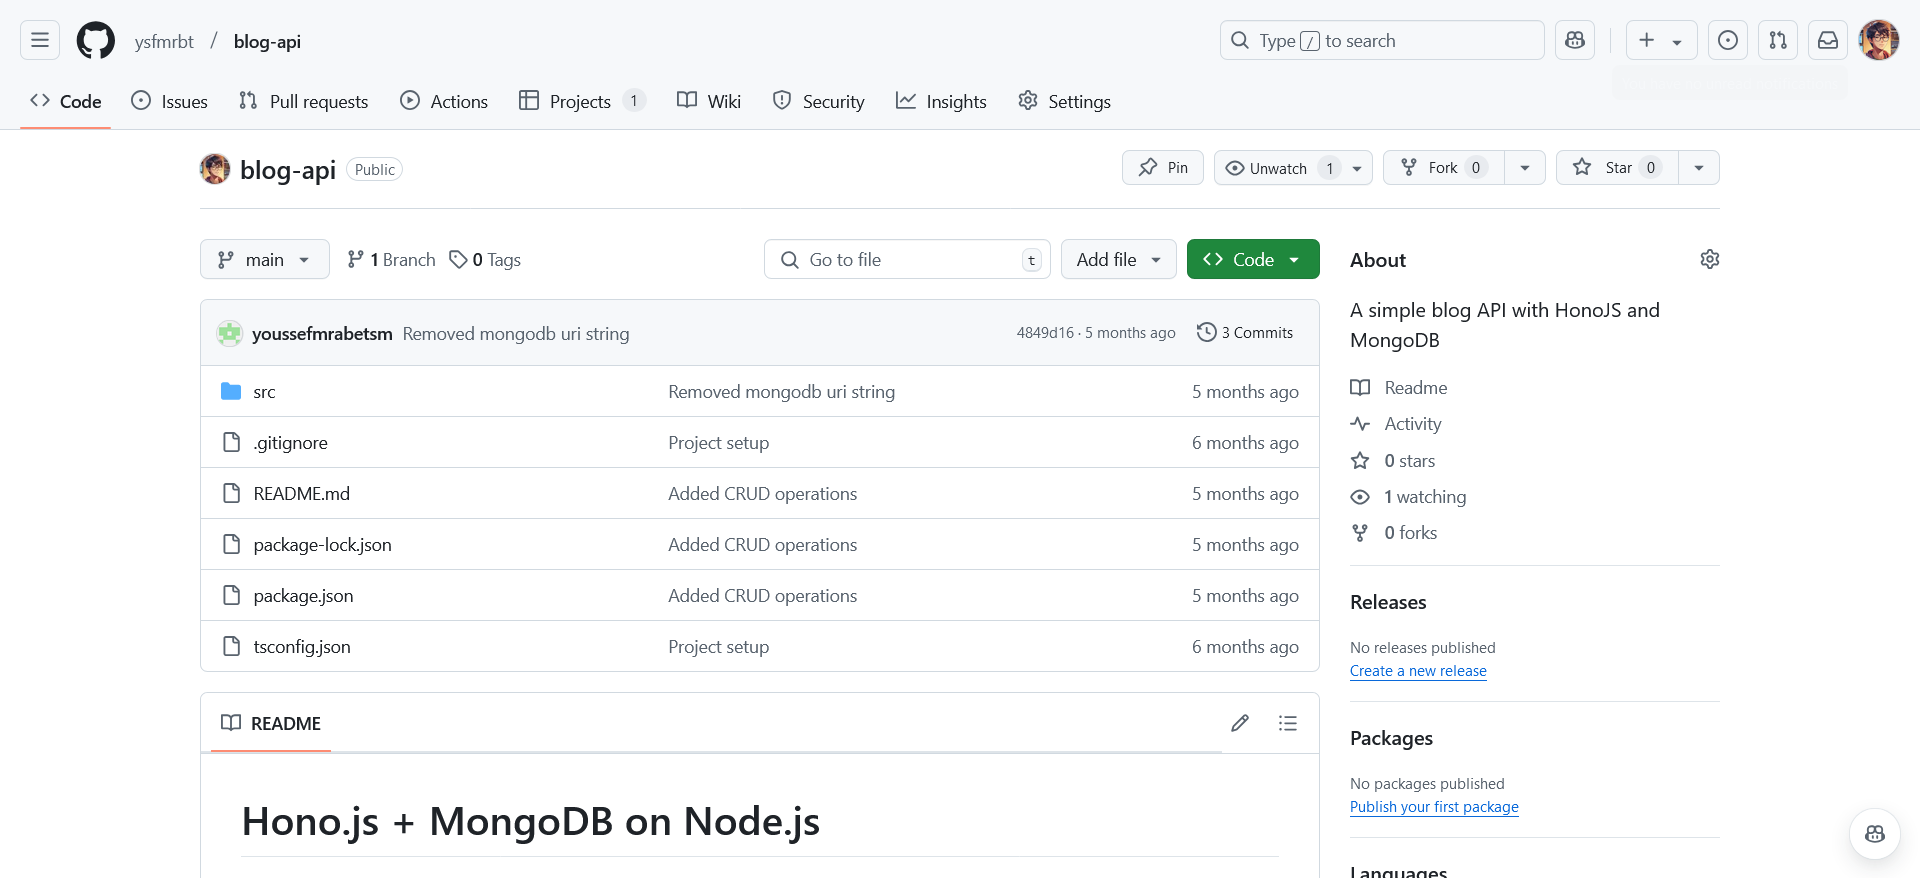
\includegraphics[width=\textwidth]{project/images/repo.png}
    \caption{An example of a GitHub repository.}
    \label{fig:github-repo}
\end{figure}
\subsubsection{GitHub Actions}
GitHub Actions is a continuous integration and continuous delivery (CI/CD) platform that allows you to automate your build, test, and deployment pipeline. \cite{ghactions}

GitHub Actions automated the execution of Playwright scripts, providing immediate feedback on code changes during sprints.

\begin{figure}[H]
    \centering
    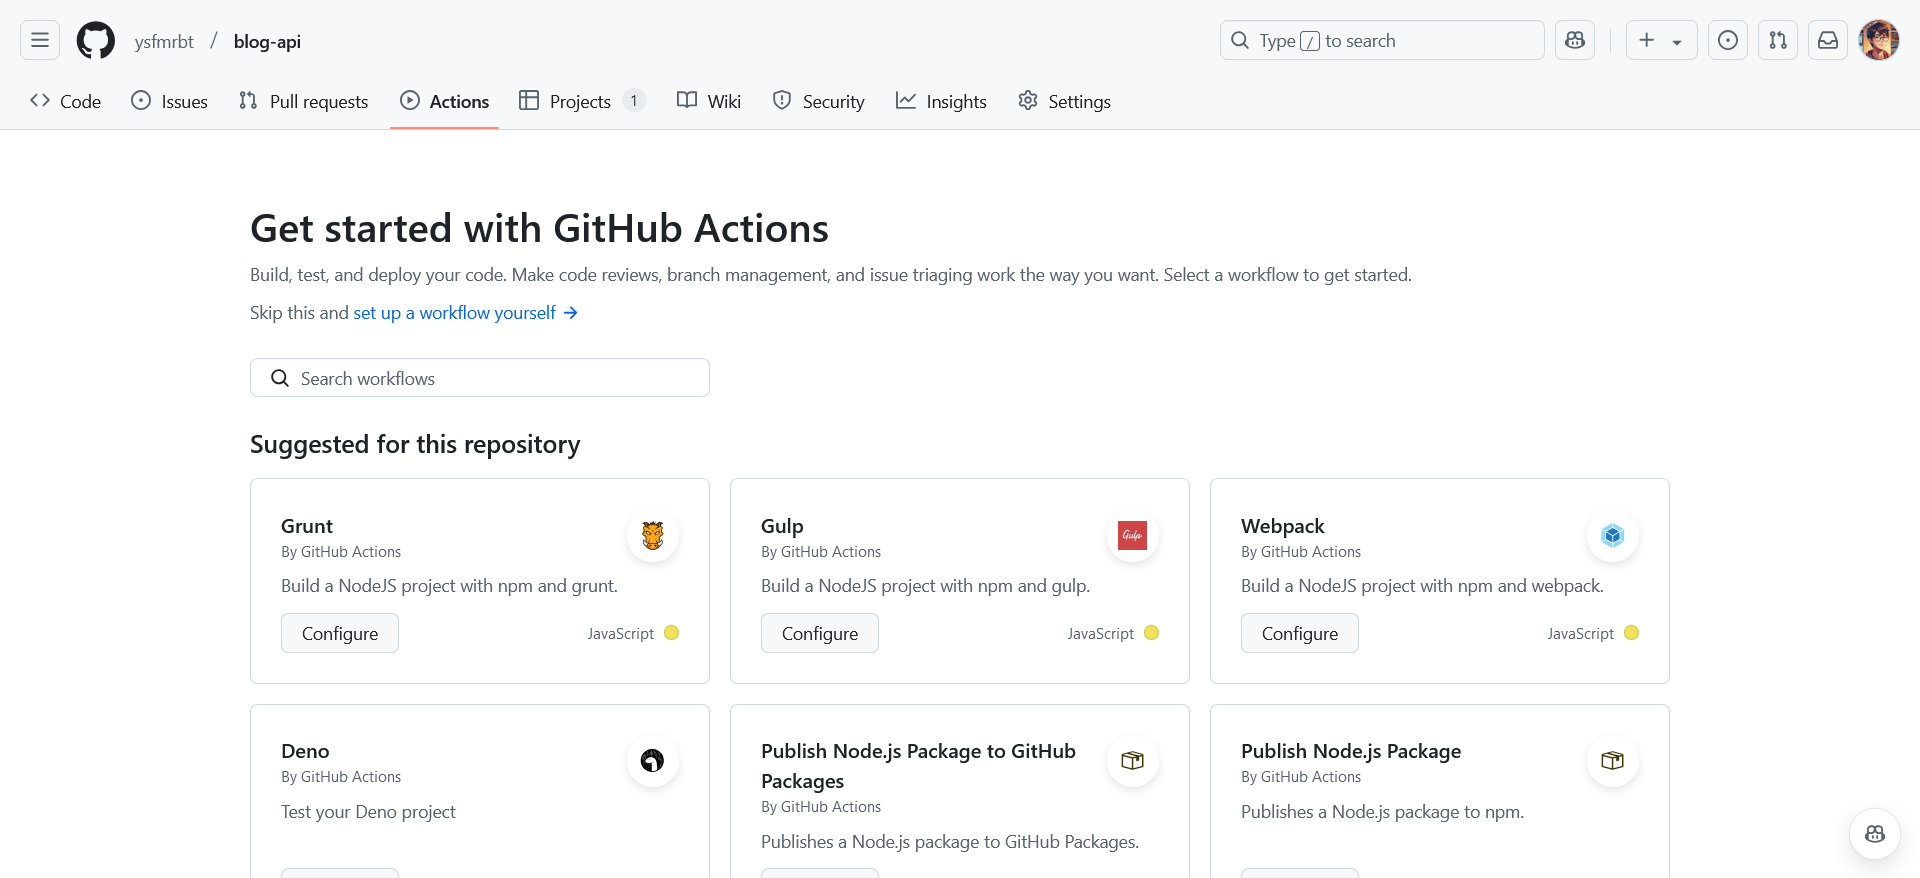
\includegraphics[width=\textwidth]{project/images/actions.png}
    \caption{GitHub Actions.}
    \label{fig:github-actions}
\end{figure}

\subsubsection{GitHub Projects}
Projects is an adaptable, flexible tool for planning and tracking work on GitHub. \cite{ghprojects}

At SeekMake, GitHub Projects was used to manage the testing process, track defects, and collaborate on testing activities.

\begin{figure}[H]
    \centering
    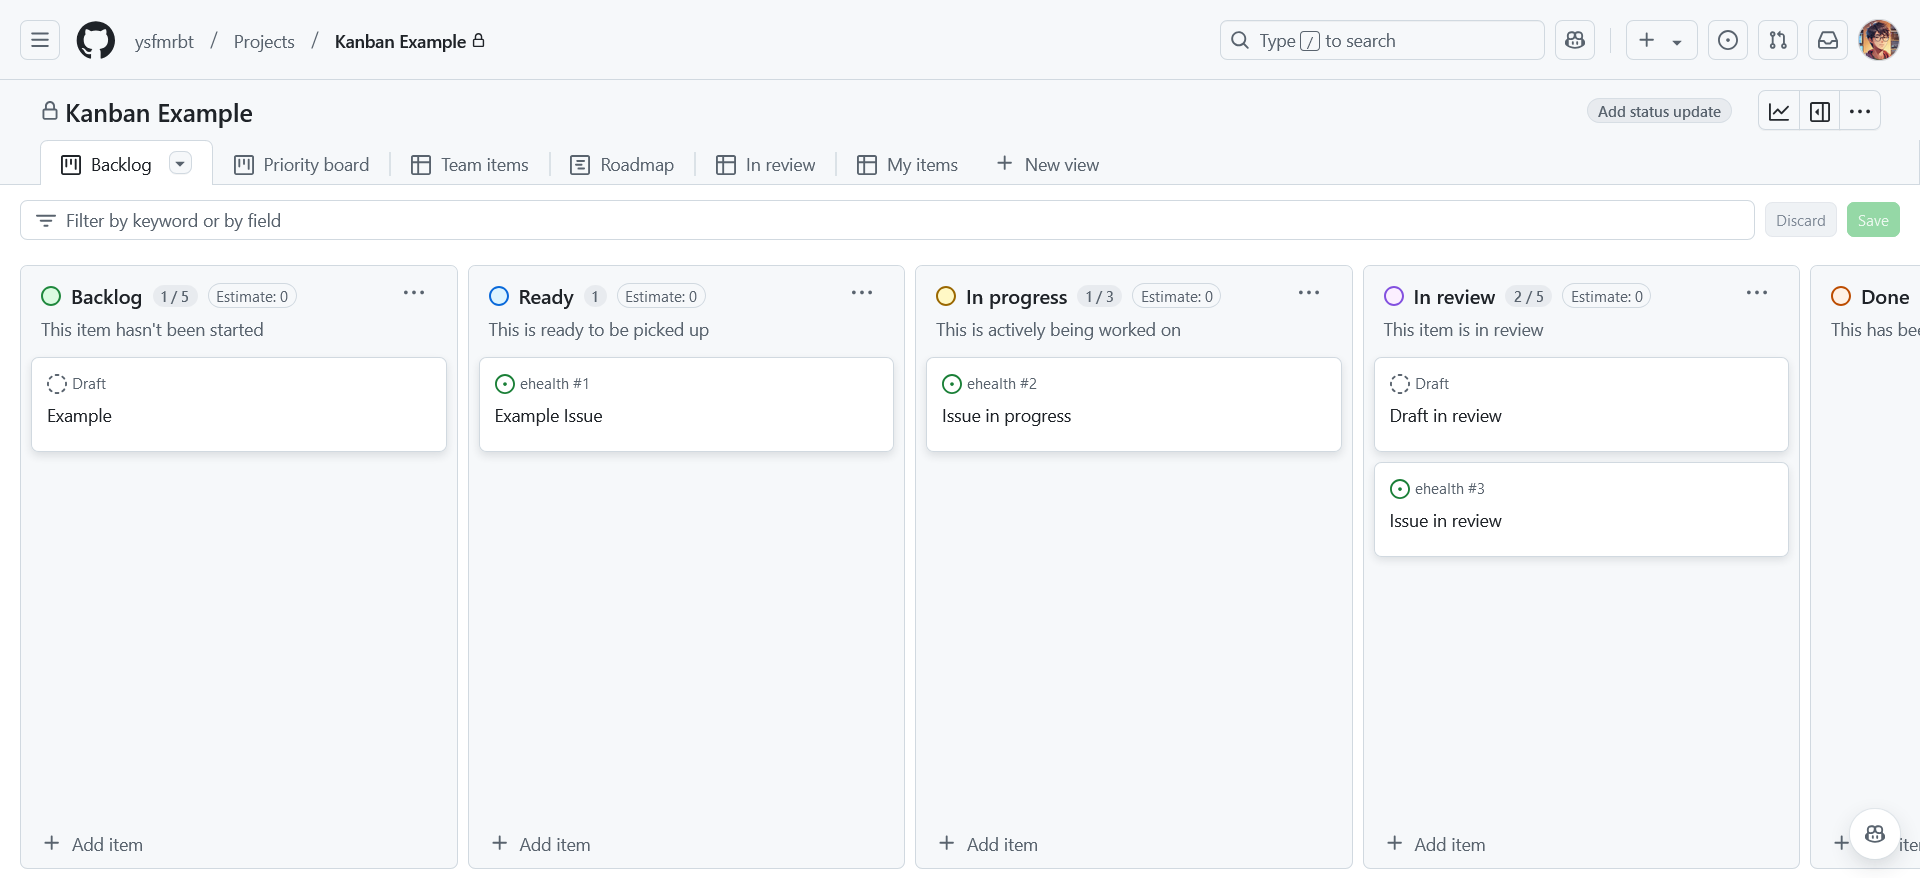
\includegraphics[width=\textwidth]{project/images/kanban.png}
    \caption{A GitHub project board resembling the Kanban board used at SeekMake.}
    \label{fig:github-kanban}
\end{figure}

\subsection{Playwright}
Playwright is a testing framework that enables reliable end-to-end testing for modern web apps \cite{pwhp}. It was created specifically to accommodate the needs of end-to-end testing. Playwright supports all modern rendering engines including Chromium, WebKit, and Firefox. Test on Windows, Linux, and macOS, locally or on CI, headless or headed with native mobile emulation. \cite{pwdocs}

Playwright was used for end-to-end testing, enabling automation across Chromium, WebKit, and Firefox browsers. It streamlined test execution for critical paths, such as the login process and account management workflows.

\begin{figure}[H]
    \centering
    
\includegraphics[width=0.5\textwidth]{project/images/Playwright_Logo.svg.png}
    \caption{Playwright logo.}
    \label{fig:playwright-logo}
\end{figure}

\subsection{Microsoft Teams}
Microsoft Teams is a Meet, chat, call, and collaborate with communications software that makes it easy to work, plan, and innovate together. \cite{msteams}

At SeekMake, Microsoft Teams was used to communicate with team members, share updates, and collaborate on testing activities.

\begin{figure}[H]
    \centering
    \includegraphics[width=0.1\textwidth]{project/images/Microsoft_Office_Teams_(2018–present).svg.png}
    \caption{Microsoft Teams logo.}
    \label{fig:msteams-logo}
\end{figure}

\subsection{BrowserStack Live}
BrowserStack Live is a cross browser on desktop and mobile testing platform. \cite{browserstack}

At SeekMake, BrowserStack Live was used to test the web application on Apple devices.

\begin{figure}[H]
    \centering
    
\includegraphics[width=0.5\textwidth]{project/images/BrowserStack_idTaghUsQq_1.png}
    \caption{Browser Stack logo.}
    \label{fig:browserstack-logo}
\end{figure}

\subsection{Lighthouse}

Lighthouse is an open-source, automated tool to help you improve the quality of web pages. You can run it on any web page, public or requiring authentication. It has audits for performance, accessibility, progressive web apps, SEO, and more.

At SeekMake, Lighthouse was used to assess web application performance and highlight areas for improvement, such as load times and accessibility.

\begin{figure}[H]
    \centering
    
\includegraphics[width=0.1\textwidth]{project/images/lighthouse-logo_512px.png}
    \caption{Lighthouse logo.}
    \label{fig:lighthouse-logo}
\end{figure}

\section{Testing Techniques}

Test techniques support the tester in test analysis (what to test) and in test design (how to test). Test
techniques help to develop a relatively small, but sufficient, set of test cases in a systematic way. Test
techniques also help the tester to define test conditions, identify coverage items, and identify test data
during the test analysis and design. \cite{istqbctfl4.0.1}

At SeekMake, the following testing techniques were used to design test cases:

\subsection{Black-box Testing Techniques}
Black-box test techniques (also known as specification-based techniques) are based on an analysis of
the specified behavior of the test object without reference to its internal structure. Therefore, the test
cases are independent of how the software is implemented. Consequently, if the implementation
changes, but the required behavior stays the same, then the test cases are still useful. \cite{istqbctfl4.0.1}

\subsubsection{Equivalence Partitioning}
Equivalence Partitioning (EP) divides data into partitions (known as equivalence partitions) based on the
expectation that all the elements of a given partition are to be processed in the same way by the test
object. The theory behind this technique is that if a test case, that tests one value from an equivalence
partition, detects a defect, this defect should also be detected by test cases that test any other value from
the same partition. Therefore, one test for each partition is sufficient. \cite{istqbctfl4.0.1}

At SeekMake, we used equivalence partitioning to design and execute test cases that verify discounts based on intervals of quantities.

\begin{figure}[H]
    \centering
    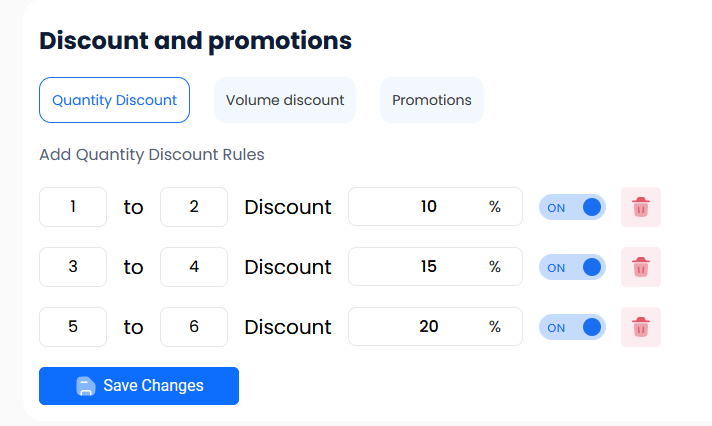
\includegraphics[width=0.5\textwidth]{project/images/ep.png}
    \caption{Screenshot taken from SeekMake's web application showing discounts based on intervals of quantities.}
    \label{fig:ep}
\end{figure}

\subsubsection{Boundary Value Analysis}
Boundary Value Analysis (BVA) is a test technique based on exercising the boundaries of equivalence
partitions. Therefore, BVA can only be used for ordered partitions. The minimum and maximum values of
a partition are its boundary values. In the case of BVA, if two elements belong to the same partition, all
elements between them must also belong to that partition. \cite{istqbctfl4.0.1}

At SeekMake, we used boundary value analysis to design and execute test cases that verify the behavior of the web application when the percentage of VAT is at the minimum and maximum values.

\begin{figure}[H]
    \centering
    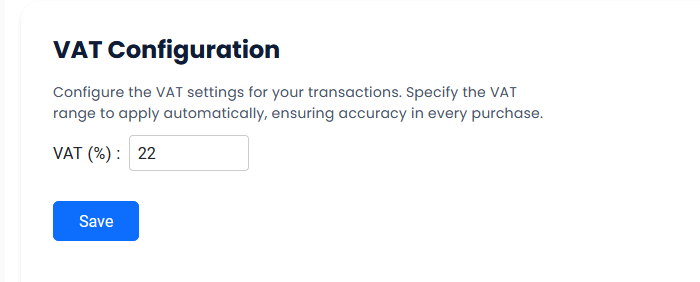
\includegraphics[width=0.5\textwidth]{project/images/bva.png}
    \caption{Screenshot taken from SeekMake's web application showing the percentage of VAT.}
    \label{fig:bva}
\end{figure}

\subsection{Experience-based Testing Techniques}
Experience-based test techniques effectively use the knowledge and experience of testers for the
design and implementation of test cases. The effectiveness of these test techniques depends heavily on
the tester’s skills. Experience-based test techniques can detect defects that may be missed using the
black-box test techniques and white-box test techniques. Hence, experience-based test techniques are
complementary to the black-box test techniques and white-box test techniques. \cite{istqbctfl4.0.1}

\subsubsection{Exploratory Testing}
In exploratory testing, tests are simultaneously designed, executed, and evaluated while the tester learns
about the test object. The testing is used to learn more about the test object, to explore it more deeply
with focused tests, and to create tests for untested areas. \cite{istqbctfl4.0.1}

At SeekMake, exploratory testing was carried out while we were learning about the web application and exploring its functionalities.
\subsubsection{Checklist-based Testing}
In checklist-based testing, a tester designs, implements, and executes tests to cover test conditions from
a checklist. Checklists can be built based on experience, knowledge about what is important for the user,
or an understanding of why and how software fails. Checklists should not contain items that can be
checked automatically, items better suited as entry criteria, exit criteria, or items that are too general
(Brykczynski 1999). \cite{istqbctfl4.0.1}

\begin{figure}[H]
    \centering
    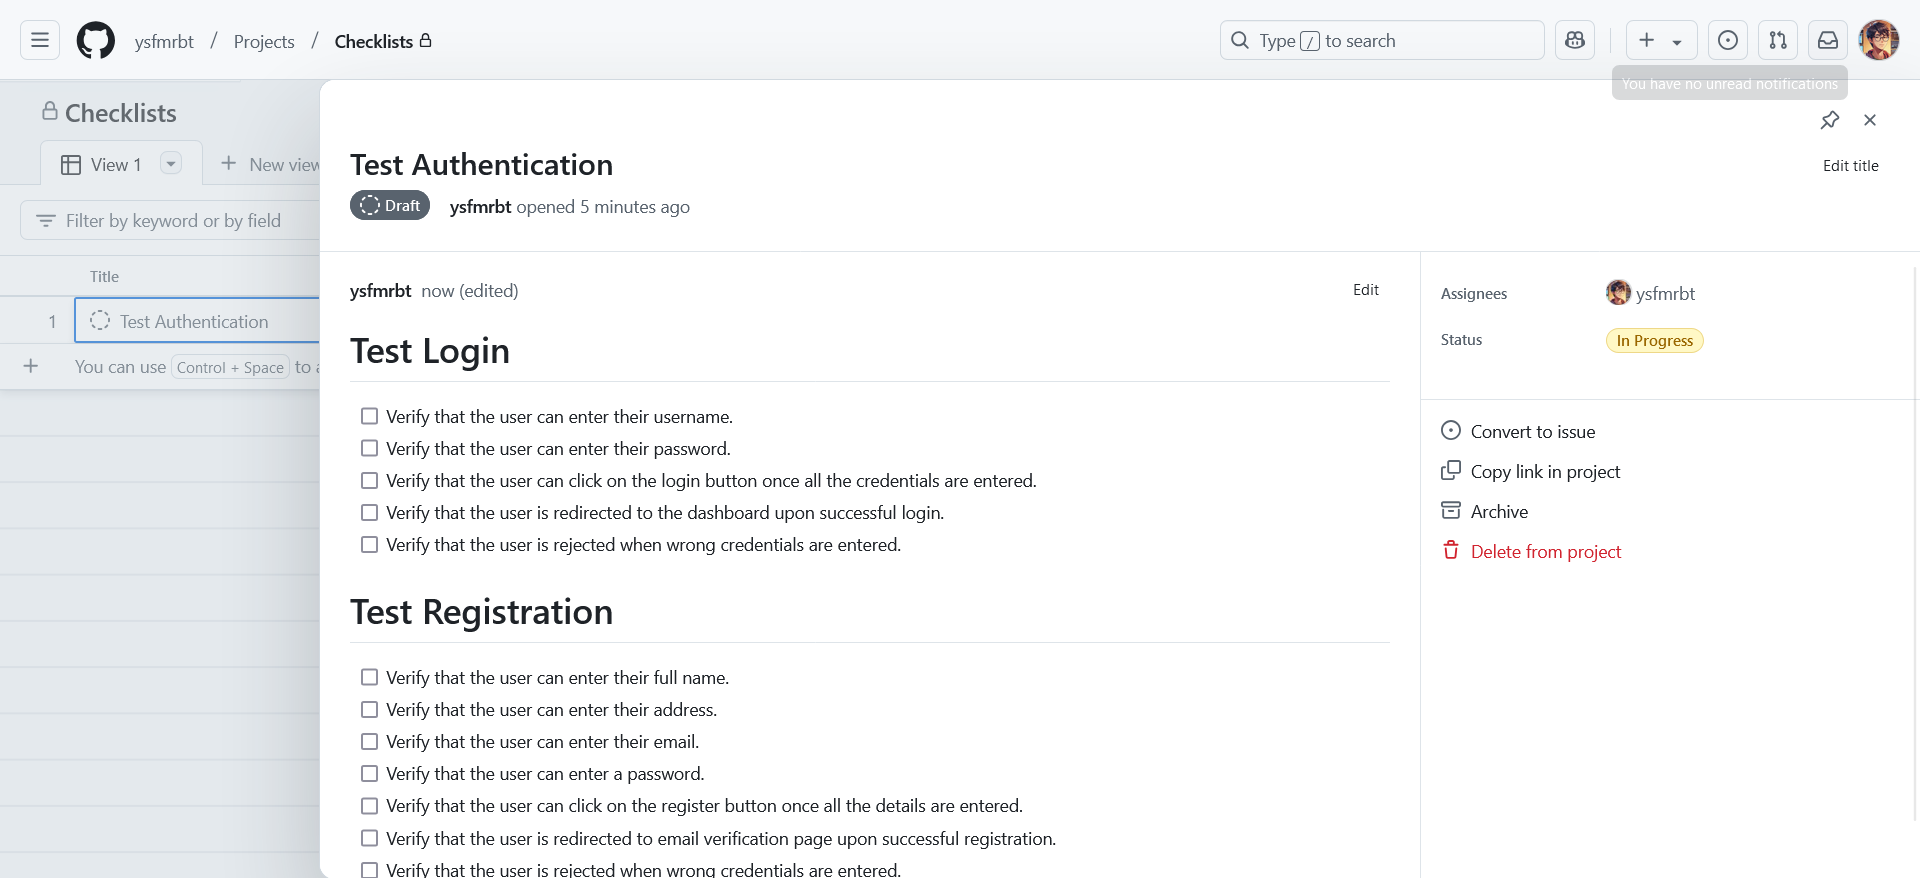
\includegraphics[width=\textwidth]{project/images/checklist.png}
    \caption{An example checklist used for Checklist-based testing at SeekMake.}
    \label{fig:gh-checklist}
\end{figure}

At SeekMake, checklist-based testing was carried out to ensure that all test conditions were covered during the testing process. We used the insights gained from exploratory testing to create checklists for future testing activities.

\section{Summary}
This chapter presented the methodology used during the software testing process at SeekMake. It included the testing strategy, testing types, testing tools, and testing techniques used to ensure the quality of the software.

The testing process was aligned with the Scrum methodology, and various testing tools were used to manage the testing process, automate testing activities, and track defects.

The testing techniques used to design test cases included black-box testing techniques and experience-based testing techniques.

The testing activities were carried out in parallel with the development activities to ensure that the software was thoroughly tested before each release.

In the next chapters, we will present how the sprints were carried out during the internship, the testing activities performed, and the results obtained.
\chapter{Exploratory Testing Insights}
\markboth{Exploratory Testing Insights}{}

\section{Introduction}
This chapter presents the first two sprints carried out during the internship at SeekMake. The sprints were focused on exploratory testing of the web application.

\section{Background}

At the beginning of the first sprint, the team was introduced to the SeekMake web application.

The team was given a brief overview of the application and its functionalities. The team was also provided with access to the application and the necessary documentation.

\section{Testing Approach}
The QA team used exploratory testing to test the SeekMake web application. The QA team explored the application without any pre-defined test cases or scripts. The team used their knowledge and experience to test the application and identify any issues or bugs.

\subsection{Micro Frontends Architecture}

The SeekMake web application is built using the Micro Frontends architecture.

The idea behind Micro Frontends is to think about a website or web app as a composition of features which are owned by independent teams. Each team has a distinct area of business or mission it cares about and specialises in. A team is cross functional and develops its features end-to-end, from database to user interface. \cite{microfrontends}

\begin{figure}[H]
    \centering
    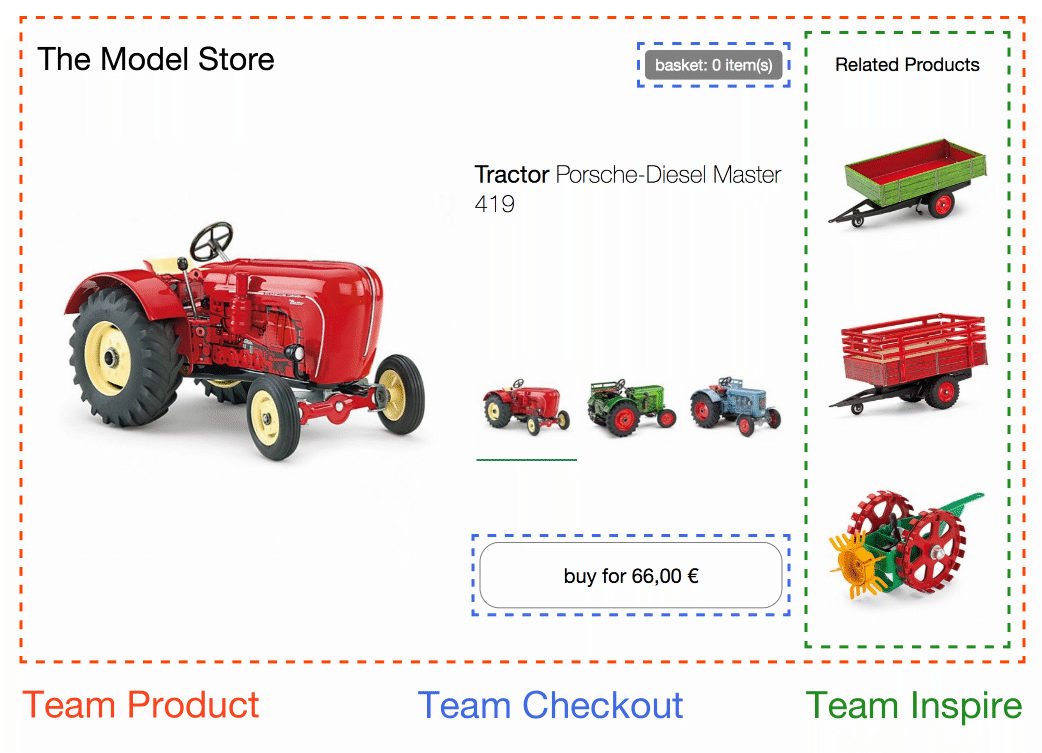
\includegraphics[width=0.8\textwidth]{project/images/three-teams.png}
    \caption{A figure demonstrating an example of Micro Frontends Architecture}
    \label{fig:microfrontends}
\end{figure}

This architecture allows the development team to work on different parts of the application independently, without affecting other parts of the application. It also allows the team to scale the application easily by adding new Micro Frontends.

The QA team was tasked with exploring the Micro Frontends of the application and identifying any issues or bugs. The team was also asked to provide feedback on the usability and user experience of the application.

\subsection{Checklists}
The QA team created checklists to guide the exploratory testing of the Micro Frontends, where each checklist focused on a specific Micro Frontend.

The checklists included a list of features and functionalities that needed to be tested, as well as a list of common issues and bugs that could be encountered.

\subsubsection{GitHub Issues}

The QA team used GitHub Issues to track bugs and issues identified during the exploratory testing.

The team created a new issue for each bug or issue identified, and assigned it to the relevant team member.

The team then worked together using collaboration tools like Microsoft Teams to resolve the issue and verify the fix.

\begin{figure}[H]
    \centering
    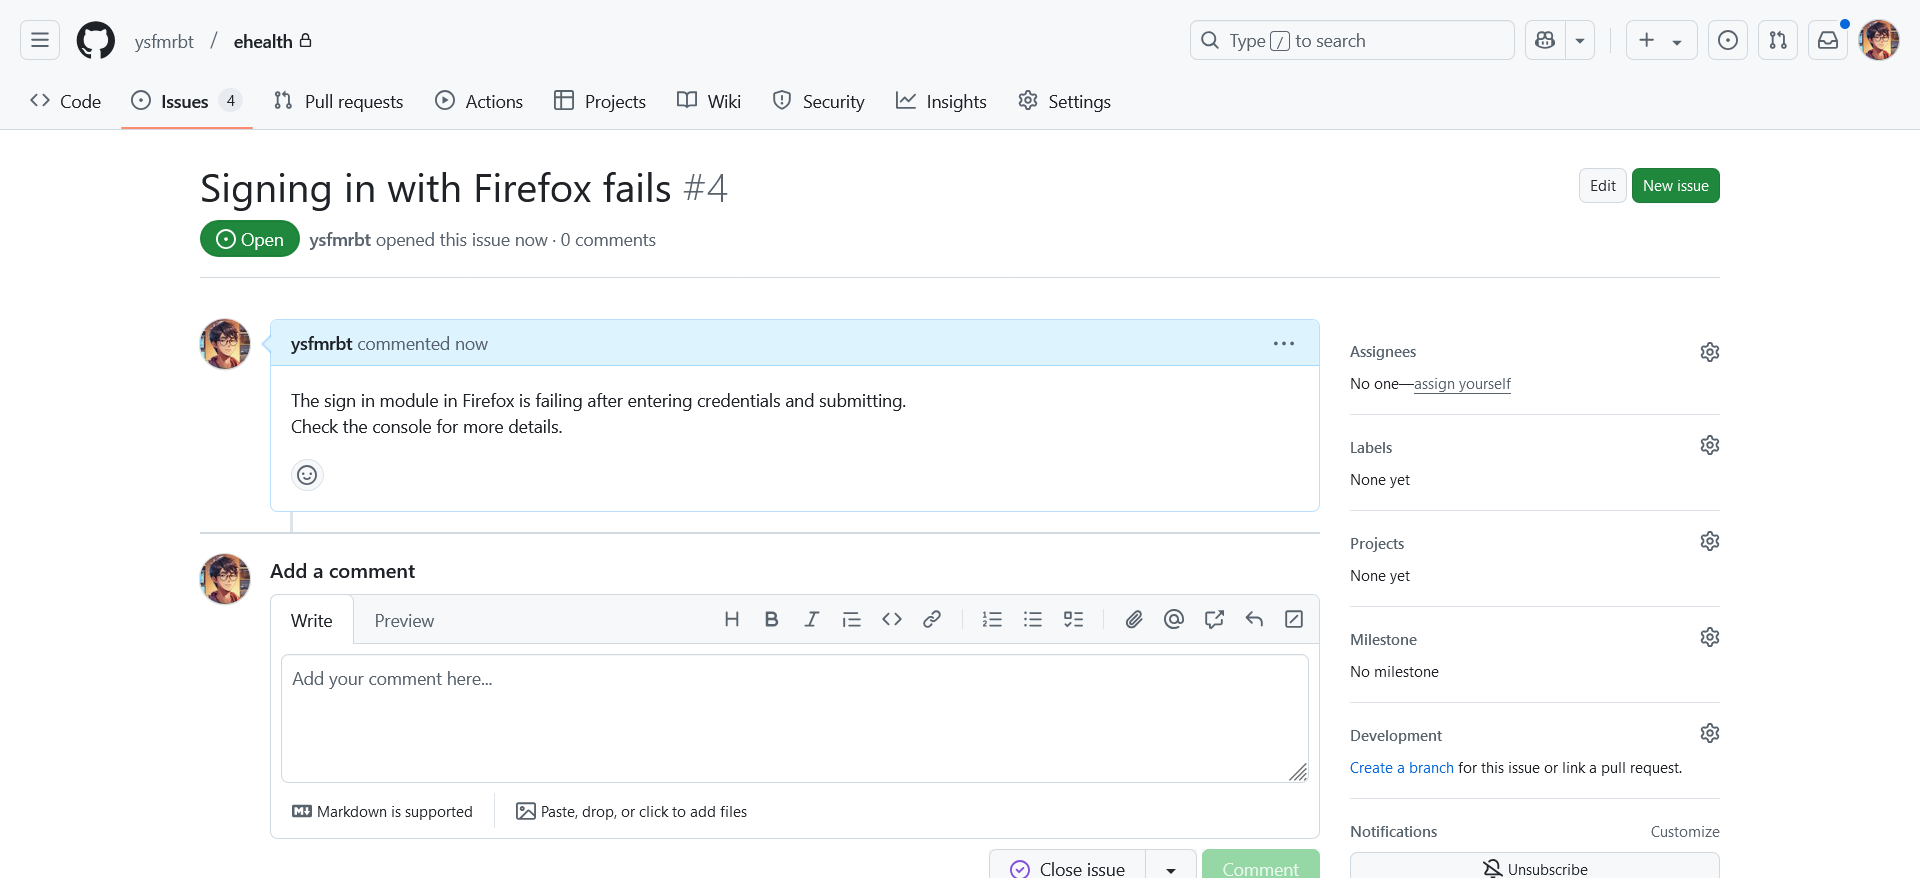
\includegraphics[width=\textwidth]{project/images/github-issue.png}
    \caption{An example of a GitHub Issue.}
    \label{fig:github-issue}
\end{figure}

The use of GitHub Issues allowed the team to track the progress of bug fixes and ensure that all issues were resolved before the end of the sprints.

\subsubsection{Confirmation Testing}

Confirmation testing confirms that an original defect has been successfully fixed. \cite{istqbctfl4.0.1}

Depending on the risk, one can test the fixed version of the software in several ways, including executing all tests that previously have failed due to the defect, or, also by adding new tests to cover any changes that were needed to fix the defect.  \cite{istqbctfl4.0.1}

The QA team performed confirmation testing to verify that all bugs and issues identified during the exploratory testing had been resolved.

\begin{figure}[H]
    \centering
    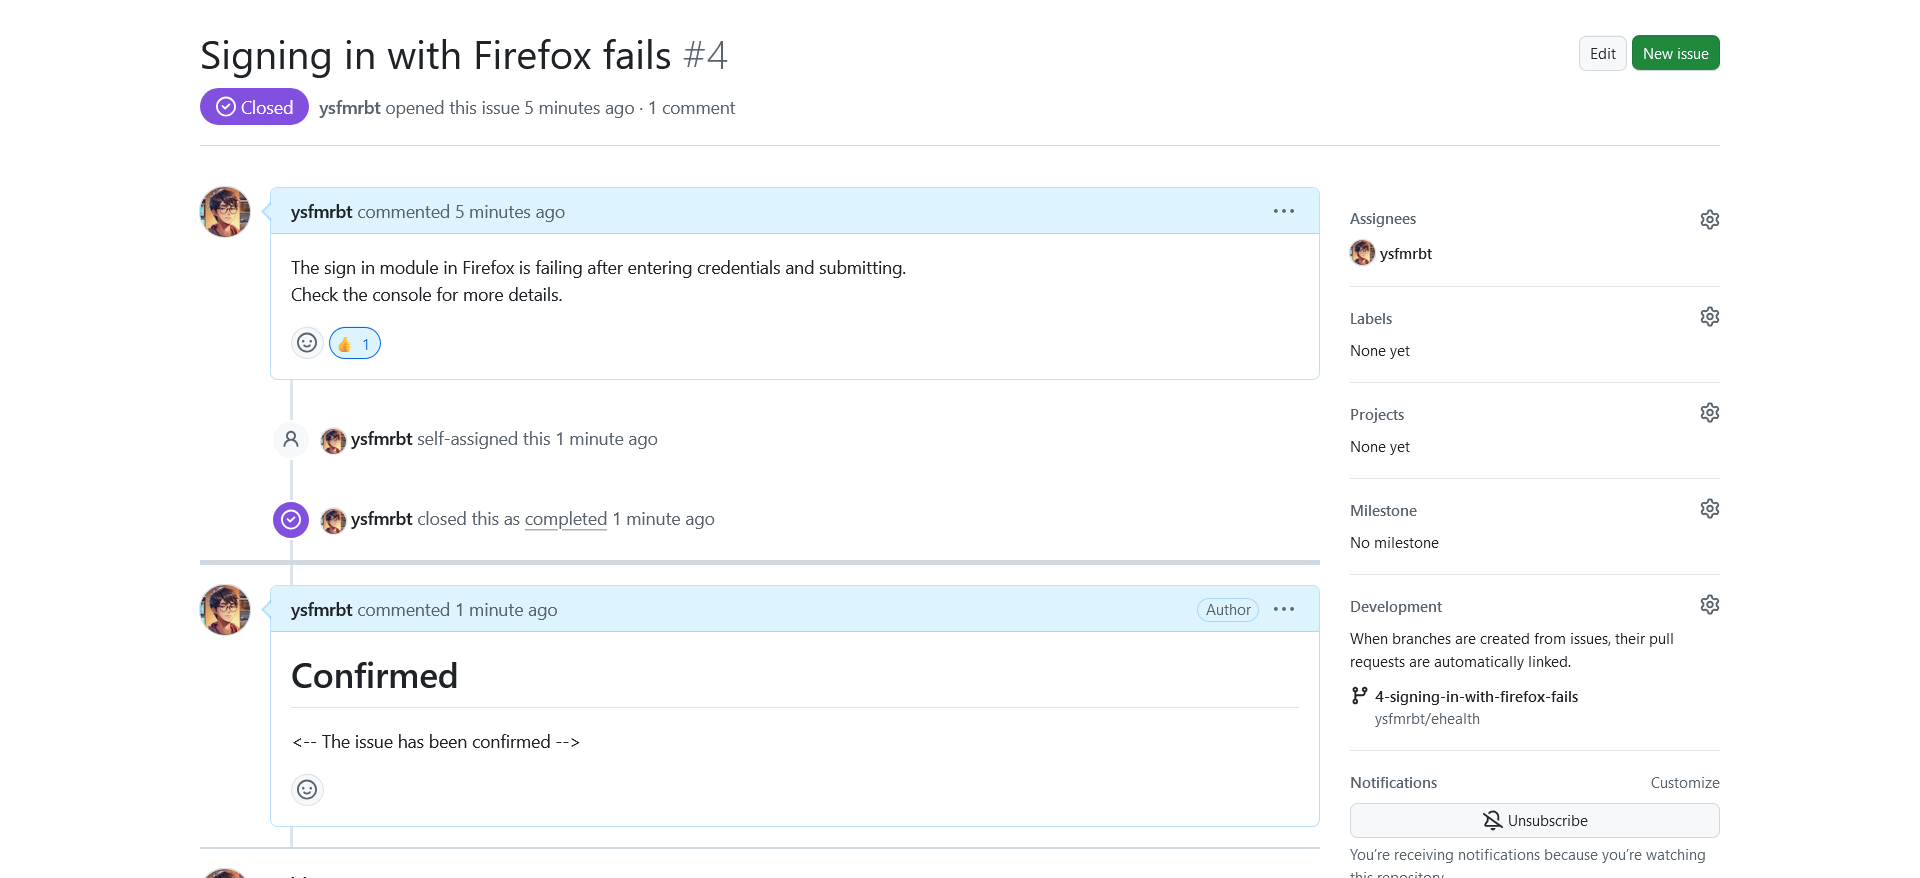
\includegraphics[width=\textwidth]{project/images/issue-confirmed.png}
    \caption{Issue confirmation.}
    \label{fig:issue-confirmed}
\end{figure}

To submit a confirmation test, the QA team followed these steps:

\begin{enumerate}
    \item Comment on the GitHub issue where the problem was reported.
    \item Attach a media (image or video) demonstrating the resolution of the problem.
    \item Close the issue to mark it as completed.
\end{enumerate}

\subsubsection{Manual Regression Testing}

Regression testing confirms that no adverse consequences have been caused by a change, including a fix that has already been confirmation tested. These adverse consequences could affect the same component where the change was made, other components in the same system, or even other connected systems. \cite{istqbctfl4.0.1}

The QA team performed manual regression testing to ensure that the bug fixes did not introduce any new issues or bugs.

\begin{figure}[H]
    \centering
    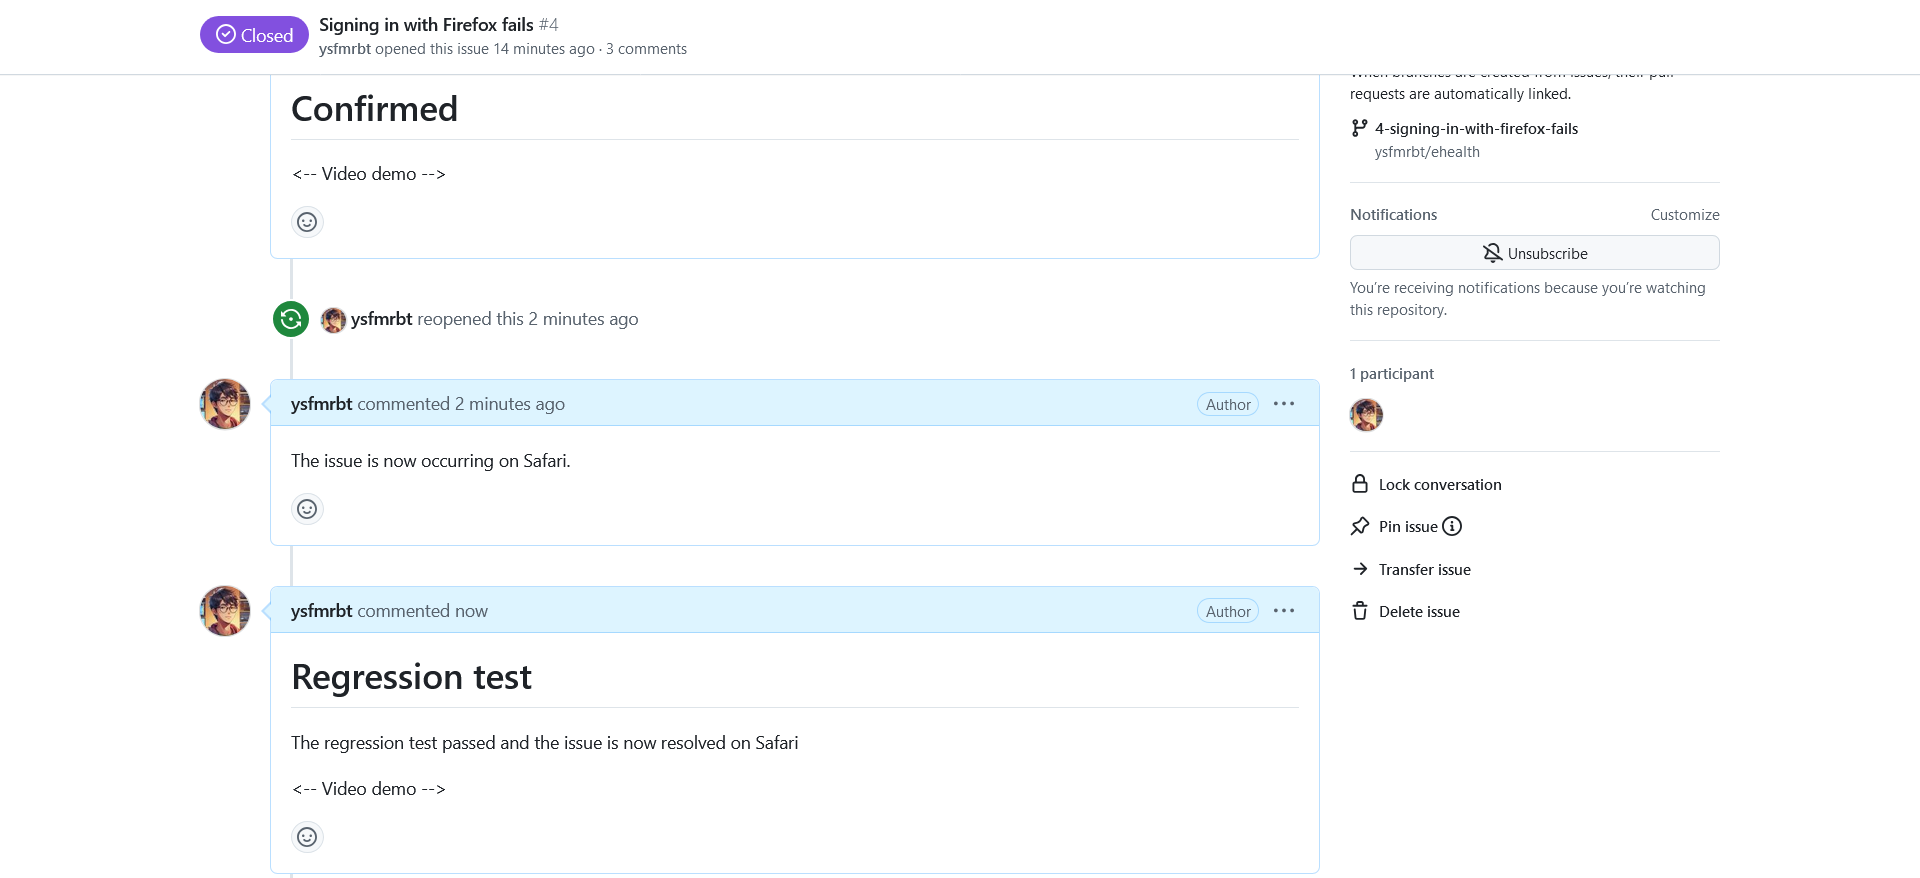
\includegraphics[width=\textwidth]{project/images/regression-test.png}
    \caption{Regression test.}
    \label{fig:regression-test}
\end{figure}

In the same way, to submit a manual regression test, the QA team followed these steps:

\begin{enumerate}
    \item Re-comment on and open the the GitHub issue where the problem was originally confirmed as resolved.
    \item Attach a media (image or video) demonstrating the resolution of the problem.
    \item Close the issue to mark it as completed.
\end{enumerate}
\section{Web Application Environment}

The SeekMake web application was deployed in different environments, including:

\subsection{Production}

The production environment is the live environment where the application is accessed by users. The production environment is deployed for using the application in a real-world scenario, and is monitored for performance and stability.

At the end of the sprints, the QA team deployed the application to the production environment for user acceptance testing.

The QA team used the production environment to test the application in a real-world scenario, and to identify any issues or bugs that were not present in the staging environment.

\subsection{Staging}

The staging environment is used for testing the application before it is deployed to production. The staging environment is an exact replica of the production environment, with the same configuration and data.

The QA team used the staging environment to test the application and identify any issues or bugs before it was deployed to production.

\subsection{Development}

The development environment is used by the development team to work on new features and bug fixes. The development environment is separate from the staging and production environments, and is used for testing changes before they are merged into the staging environment.

The QA team used the development environment to test new features and bug fixes before they were deployed to staging.

\section{Testing Results}

The QA team identified several bugs and issues during the exploratory testing of the SeekMake web application.

The bugs and issues were prioritised based on their severity and impact on the application and users. The team worked together to resolve the bugs and issues before the end of the sprints.

\subsection{Bugs and Issues}

The bugs and issues identified during the exploratory testing included:

\begin{itemize}
    \item Broken links (e.g. links that do not work or lead to the wrong page)
          Two examples of broken links are:
          \begin{itemize}
              \item The "Contact Us" link on the homepage redirected to the "About Us" page.
              \item The "Terms and Conditions" link on the checkout page redirected to a 404 error page.
          \end{itemize}
    \item Incorrect data (e.g. data that is missing or incorrect)
          \begin{figure}[H]
              \centering
              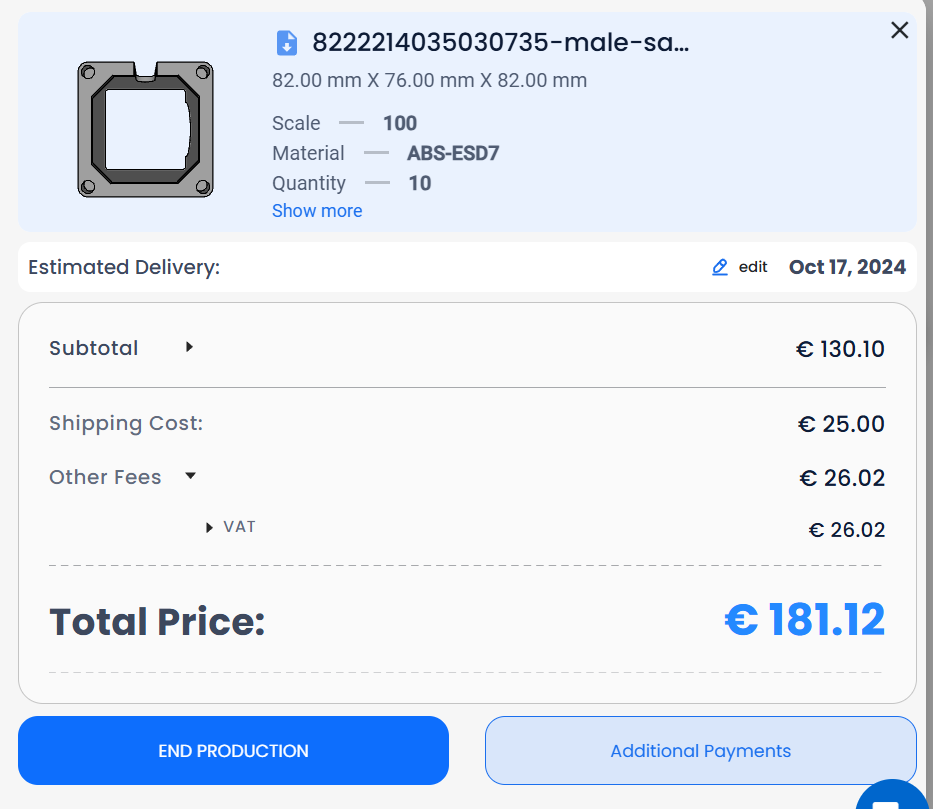
\includegraphics[width=0.5\textwidth]{project/images/incorrect-data.png}
              \caption{An example of incorrect data (Total price should be 181.02 instead of 181.12).}
              \label{fig:incorrect-data}
          \end{figure}
    \item Missing features (e.g. features that are not implemented or are not working as expected). An example of a missing feature that was encountered in SeekMake, is that users from certain countries were not able to complete the payment process.
    \item Performance issues (e.g. slow loading times or unresponsive pages). At the start of the sprint, the application took 10 seconds on average to load the homepage. After the sprint, the application took 5 seconds on average to load the homepage.
    \item Usability issues (e.g. poor navigation, confusing layout)
          \begin{figure}[H]
              \centering
              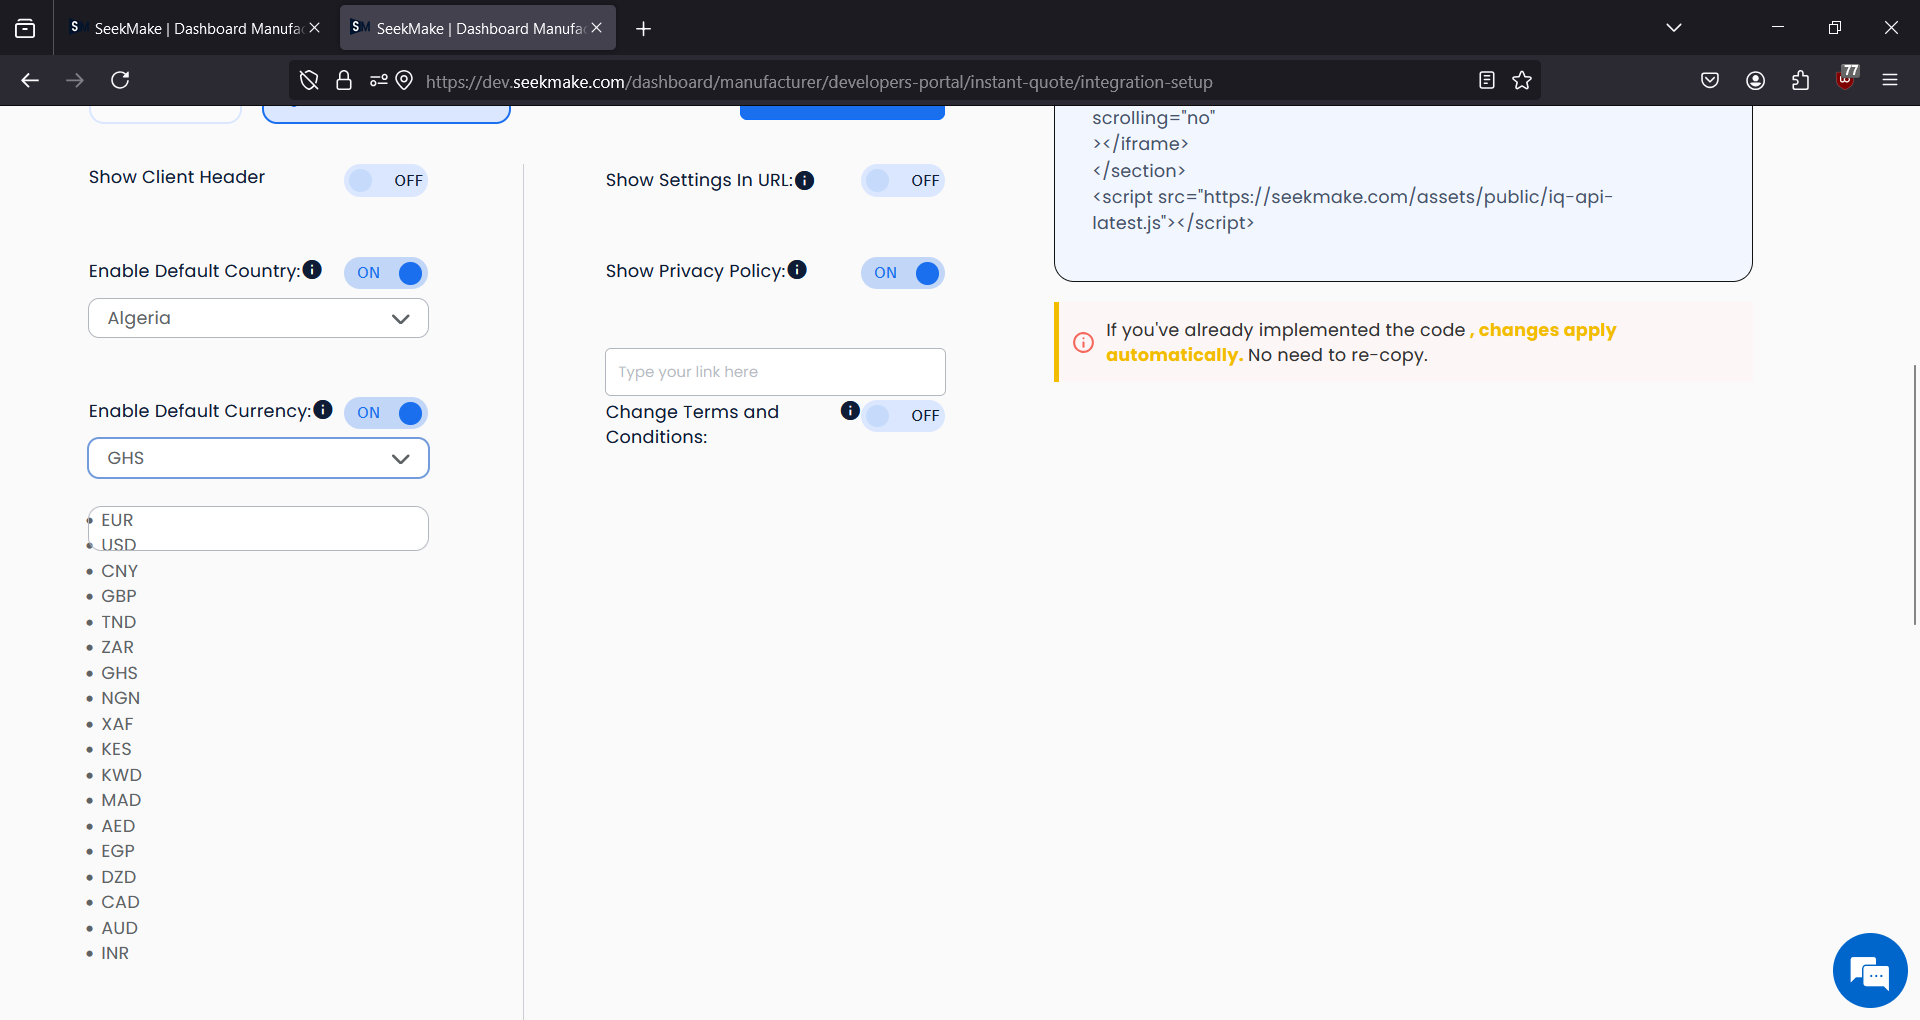
\includegraphics[width=\textwidth]{project/images/dropdown-broken.png}
              \caption{An example of a dropdown not fully implemented.}
              \label{fig:dropdown-broken}
          \end{figure}
    \item Security vulnerabilities (e.g. unprotected data). At the start of the sprint, a user could access the manufacturer dashboard by changing the URL. After the sprint, the manufacturer dashboard required the user to switch to a manufacturer account.
    \item Compatibility issues (e.g. the application does not work on certain devices or browsers). At the start of the sprint, the application did not work properly on Safari browser. After the sprint, the application worked on Safari.
\end{itemize}

The following are examples of how the bugs and issues were prioritised:
\begin{itemize}
    \item Critical: Payment gateway failed to process certain transactions.
    \item Major: Navigation links redirected to incorrect pages.
    \item Minor: Text alignment issues on smaller screen resolutions.
\end{itemize}
\section{Summary}

The first two sprints focused on exploratory testing of the SeekMake web application. The QA team used exploratory testing to test the Micro Frontends of the application and identify bugs and issues.

The team created checklists to guide the exploratory testing, and used GitHub Issues to track bugs and issues. The team performed confirmation testing and manual regression testing to verify that all bugs and issues were resolved.

The QA team identified several bugs and issues during the exploratory testing, and worked together to resolve them before the end of the sprints.

In the next sprint, the team will focus on end-to-end testing of the SeekMake web application.
\chapter{End-to-End Testing and Automation}
\markboth{End-to-End Testing and Automation}{}

\section{Introduction}

This chapter presents the final sprint carried out during the internship at SeekMake. The sprint was focused on end-to-end testing of the web application.

\section{E2E Testing Fundamentals}

End-to-end testing, also known as E2E testing, is an approach to testing that that simulates real user experiences to validate the complete system. \cite{circleci}

\subsection{Goals}

The primary goal of E2E testing is to ensure that the application behaves as expected from the user's perspective. E2E testing is used to validate the functionality, usability, and performance of the application.

\subsection{Benefits}

E2E testing offers several benefits, including:

\begin{itemize}
    \item Validates the complete system
    \item Identifies issues that cannot be found with unit or integration testing
    \item Provides confidence in the application's quality
    \item Reduces the risk of bugs and issues in production
\end{itemize}

\section{E2E Testing Strategy at SeekMake}

The E2E testing strategy at SeekMake was designed to validate the functionality, usability, and performance of the web application. The strategy included the following components:

\subsection{Test Environment Setup}

The QA team set up test environments to test the application in different scenarios, including production, staging, and development environments.

\subsection{Test Planning Approach}

The QA team used a risk-based approach to test planning, focusing on high-risk areas of the application. The team created test plans and test cases to guide the testing process.

\subsection{Test Case Design Methodology}

The QA team used a combination of manual and automated test cases to validate the application. The team created test cases based on user stories and acceptance criteria.

\section{Implementation with Playwright}

The QA team used Playwright, an open-source testing framework, to automate the E2E testing of the web application. Playwright provides a simple and powerful API for automating web browsers, and supports multiple programming languages, including JavaScript, Python, and C\#.

\subsection{Framework Setup}

The QA team set up the Playwright framework with Node.js to automate the E2E testing of the web application. The framework included test scripts, test data, and test reports.

\subsection{Test Script Development}

The QA team developed test scripts to validate the functionality, usability, and performance of the web application. The team used Playwright's API to interact with the web application and verify the expected results.

\subsection{Test Execution}

The QA team executed the test scripts in different environments, including production, staging, and development environments. The team monitored the test results and reported any issues or bugs in a weekly report.

\begin{figure}[H]
    \centering
    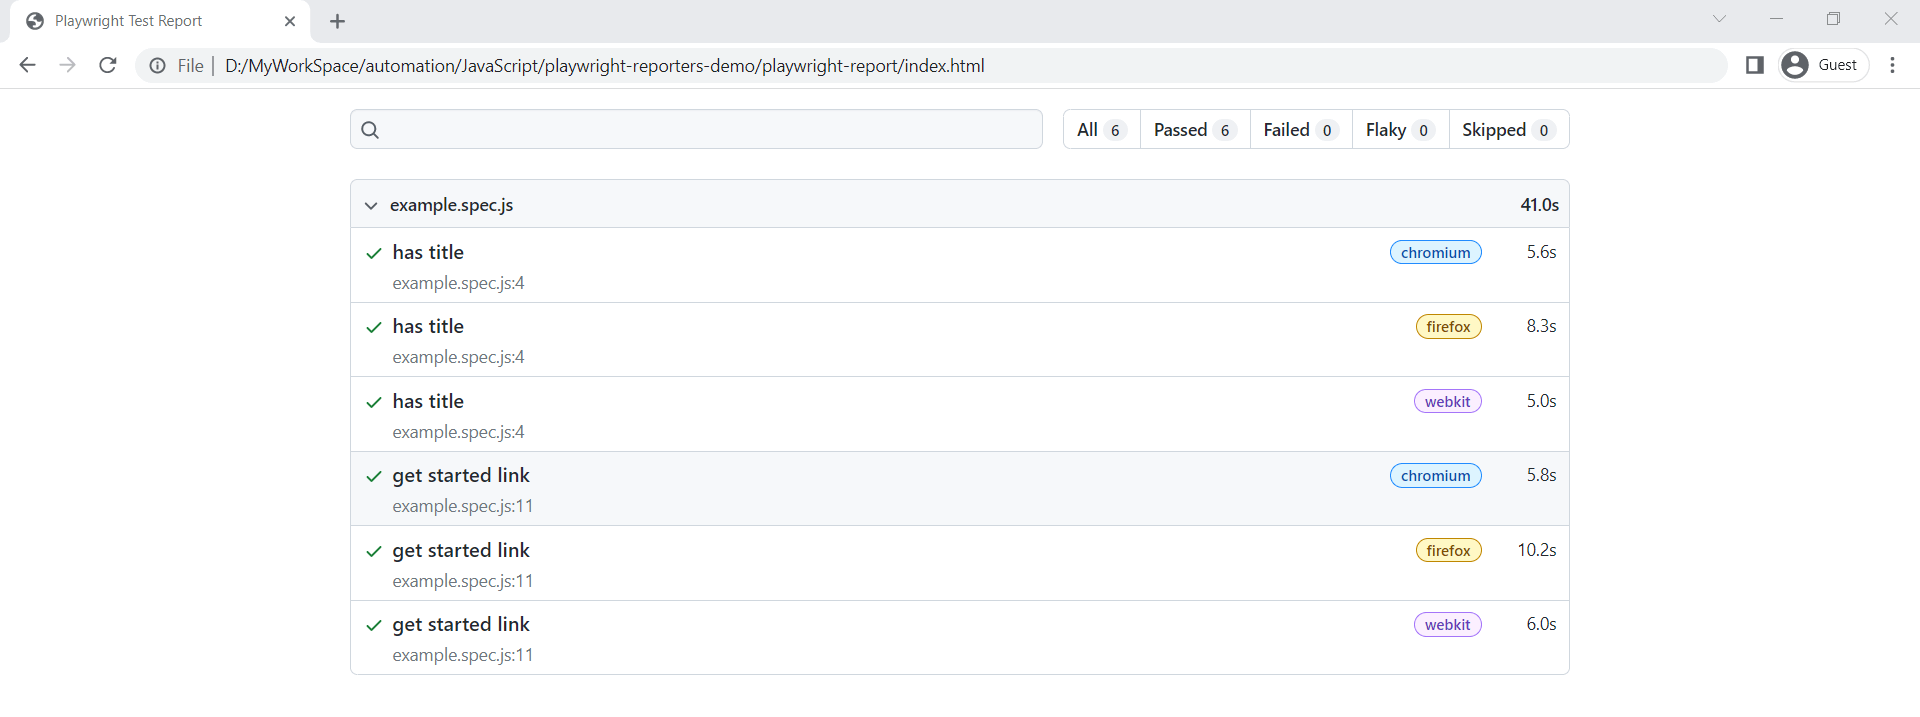
\includegraphics[width=\textwidth]{project/images/playwright-reporting-playwrightreport.png}
    \caption{An example of a Playwright report}
    \label{fig:playwright-report}
\end{figure}

\section{Results and Analysis}

End-to-end testing focused on validating critical user workflows, including account creation, login, and payment processing. Cross-browser tests conducted via BrowserStack revealed rendering inconsistencies in Safari, which were resolved through CSS optimizations. Lighthouse metrics showed significant improvements in performance, with page load times reduced by 30\% on average.
\subsection{Test Coverage}

The QA team tested all critical user journeys, such as account creation, login, and payment processing, ensuring these workflows functioned without issues across various devices and browsers.

\subsection{Cross-Browser Testing}

The QA team performed cross-browser testing to validate the application on different browsers, including Chrome and Firefox. The team identified browser-specific issues and reported them for resolution.

The team used BrowserStack Live to run the tests on Apple's Safari browser on different devices.

\subsection{Performance Considerations}

The QA team monitored the performance of the web application during the E2E testing. The team identified performance issues, such as slow loading times and unresponsive pages, and reported them for resolution.

The team used Lighthouse to measure the performance of the web application and identify opportunities for improvement.

\begin{figure}[H]
    \centering
    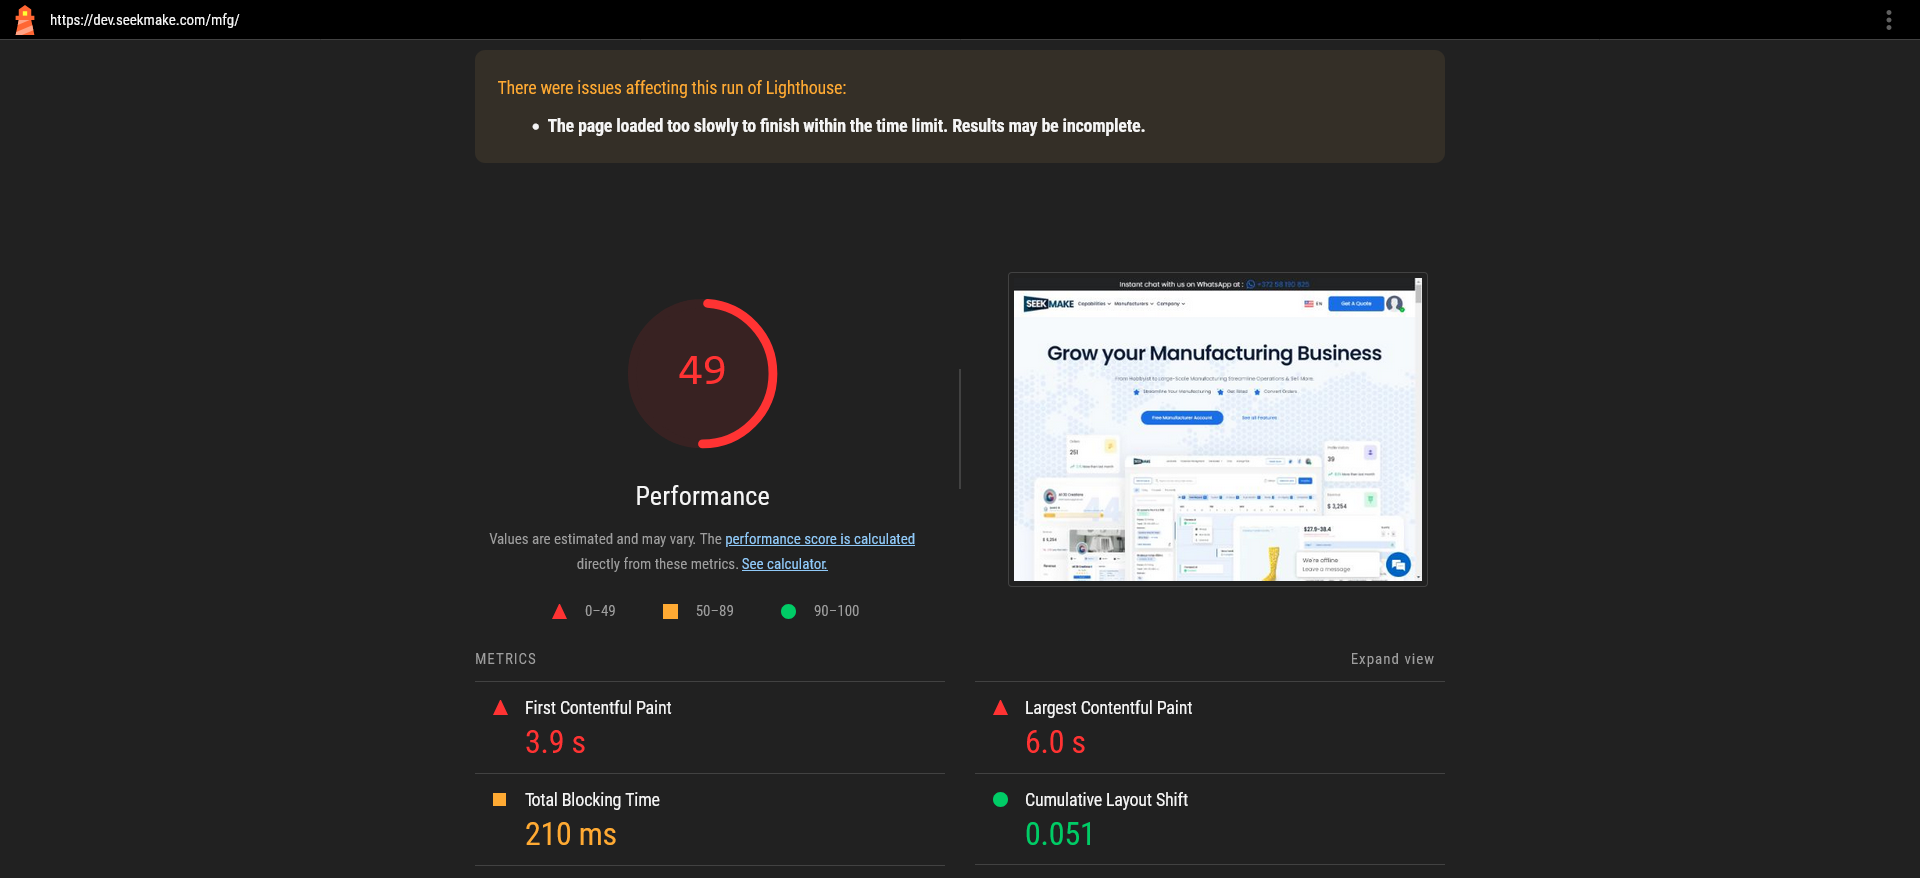
\includegraphics[width=\textwidth]{project/images/lighthouse-report.png}
    \caption{An example of a Lighthouse report}
    \label{fig:lighthouse-report}
\end{figure}

\section{CI/CD Integration}

The QA team integrated the E2E testing framework with the CI/CD pipeline to automate the testing process. The team used GitHub Actions to trigger the test execution on every code change.

\subsection{GitHub Actions Workflow}

The QA team created a GitHub Actions workflow to run the E2E tests on every pull request.

The workflow included steps to install dependencies, build the application, and run the test scripts.

\subsection{Test Automation Pipeline}

The QA team set up a test automation pipeline to automate the E2E testing of the web application.

The pipeline included stages for test execution, test reporting, and test result analysis.

\section{Summary}

The final sprint focused on end-to-end testing of the SeekMake web application. The QA team used Playwright to automate the testing process and validate the functionality, usability, and performance of the application.

The team identified several issues and bugs during the E2E testing, and reported them for resolution.

The team integrated the E2E testing framework with the CI/CD pipeline to automate the testing process. The team used GitHub Actions to trigger the test execution on every code change.

\chapter*{Summary}
\addcontentsline{toc}{chapter}{Summary}
\markboth{Summary}{}

To summarize, this report has presented the results of an internship at SeekMake, a software development company that provides digital transformation services to businesses and customers. The internship focused on software testing, with an emphasis on end-to-end testing of the web application developed by SeekMake.

The initial sprints prioritized exploratory testing to uncover functional and usability issues in the web application’s Micro Frontends architecture. The insights gained were instrumental in refining test cases for end-to-end testing during the final sprint. This iterative approach ensured that all critical workflows were thoroughly validated before deployment.

This internship was transformative, providing me with hands-on experience in test automation using Playwright and continuous integration through GitHub Actions. Collaborating with a cross-functional Agile team enhanced my communication and problem-solving skills, preparing me for future roles in software quality assurance. Additionally, the challenges of debugging cross-browser issues deepened my technical expertise in compatibility testing.
\bibliographystyle{plain}
\bibliography{software-testing}
\end{document}